\chapter{System Design}
\section{System Architecture}
\subsection{Logical Architecture}
\begin{figure}[H]
\centering
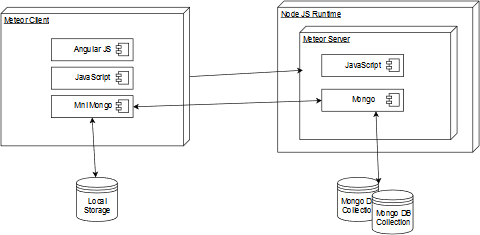
\includegraphics{Figures/LogicalArchitecture.png}
\caption{The logical architecture of the solution}
\label{fig:dataModel}
\end{figure}
We are using the Meteor framework in this project, and Meteor in turn uses the open source database MongoDB, which is different from traditional SQL databases like MySQL, PostgreSQL and OracleDB. MongoDB is a NoSQL type database. Meteor uses MongoDB in a very unique way to achieve real-time update of view layer.

Traditionally, when users interact with something on the view layer, for instance, clicking on log in or sign up button, the action triggers interaction with database sitting on the server side. This kind of interaction with the database often results in reloading of the page the user is currently on. Not only the reloading of the page is a bad user experience, it ‘eats’ bandwidth and network data because reloading of a page reloads the whole page when only a part of the page is needed to be updated.

Meteor’s way to solve this problem is by creating a mini replica of the MongoDB database on the client side. In this mini-Mongo database, partial data that users need to interact, are stored. Since mini-Mongo database resides on the user side, interactions happen in real time which means data is updated almost constantly without the page needing to reload at all. This feature enables smooth interaction on the view layer and users do not need to wait long for a response from the server. To better illustrate this feature, please see the below diagram for the overall architecture of Meteor framework. 

\subsection{Physical Deployment}

The web solution and app have different ways of being deployed, and we will walk you through these in the following sections.
\subsubsection{Web solution}
The website may be deployed in a variety of ways, but SINTEF wanted us to enable a specific mode of deployment, so that is what we have done.

The solution used to deploy the website is by packaging the project into a Docker container. This container manages the website and all its dependencies. For more info on how this works see the Docker web page \cite{docker}.

As previously explained this is done by packaging our website into a Docker container by adding a Dockerfile with info relevant to the website and its dependencies. The website is then deployed to a virtual Docker machine that can be deployed to a server. This allows for multiple solutions being run at a single server.

\subsubsection{App solution}
The App and its deployment is limited to the deployment channels of Apple and Google Play. Cordova is the app component that manages the build process of the apps to allow for deployment through these channels.

There are some restrictions as to who, how and what is allowed through the deployment channels of Apple and Google. One example is the \$100 yearly fee of being an registered Apple developer, and the \$25 one-time fee of being an registered Google developer.

In order to deploy an app to the App Store you need to go through Xcode. You can either upload the app directly from Xcode or archive it and add it through iTunes Connect. It takes a while for the app to be approved as Apple does rigorous testing of the app before releasing it.

Deploying to Google Play is a lot easier. You build an APK file and upload it to Google Play.
\section{System Components}
\subsection{Data Model}
Our solution has three main entities. These are users, events and exercises. Events can be created by both users and administrators, they are fixed to certain dates and times, and creators of events can invite friends to these events. Exercises, on the other hand, are URLs pointing to exercise videos. They are not fixed to any date or location, nor can one invite friends to join exercises. Exercises can only be added to the system by administrators. Exercises can also be included in events, but not vice versa. Figure \ref{fig:dataModel} describes the data model and shows how the different entities are related.
\begin{figure}[H]
\centering
\includegraphics[scale=0.5]{Figures/Datamodel.png}
\caption{Data model of the solution}
\label{fig:dataModel}
\end{figure}

\subsection{Class Diagram}
\begin{figure}[H]
\centering
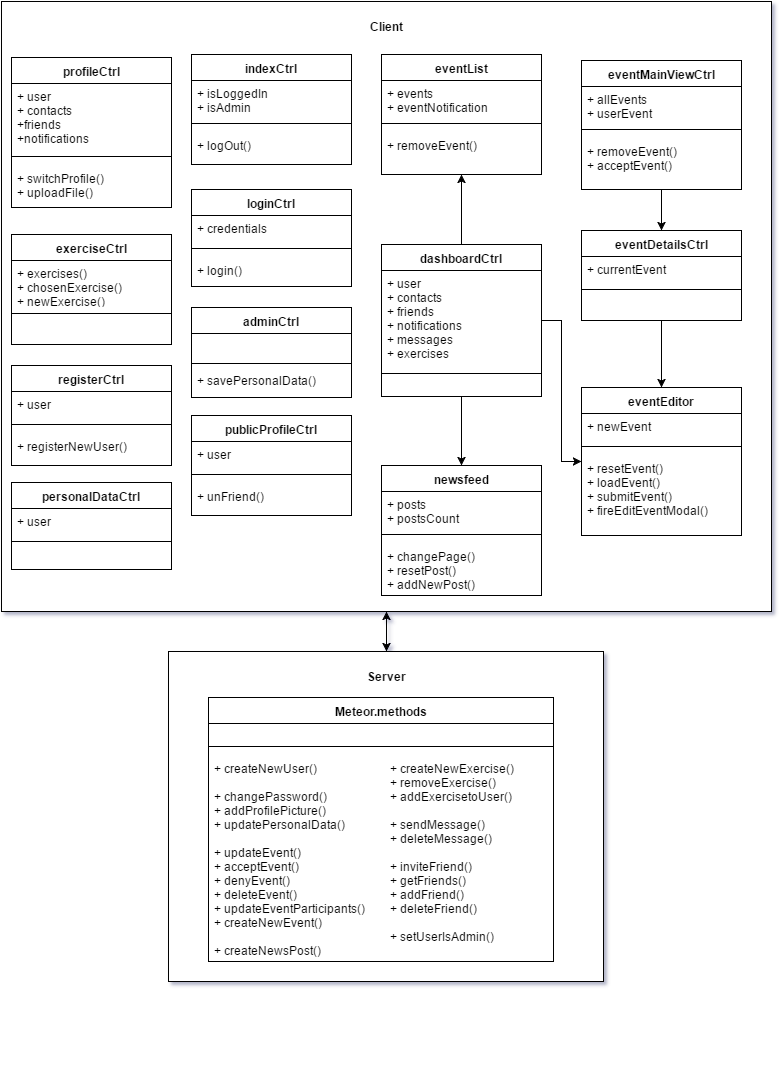
\includegraphics[scale=0.6]{Figures/ClassDiagram.png}
\caption{Class diagram of the components in the solution}
\label{fig:classDiagram}
\end{figure}
Because Angular Meteor encourages us to not use the traditional class-object format of Object-Oriented Programming, we chose to use a similarly non-traditional class diagram. Each of the methods in the server is simply saved in a "Meteor.methods" object. Furthermore, each of the controllers (and directives) are separately connected to a HTML-template and optionally URL. This is why most of the client-side classes are not connected to each other, and a simple arrow is used for those employing any manner of inheritance.

\subsection{Sequence Diagrams}
\begin{figure}[H]
\centering
  \includegraphics[width=0.5\linewidth]{Figures/seqDiagramRegister.png}
  \caption{Sequence Diagram for Use Case 1, see Table \ref{fig:UC1}}
  \label{fig:SeqDig1}
  \end{figure}

\begin{figure}[H]
  \centering
  \includegraphics[width=0.5\linewidth]{Figures/seqDiagramCreateEvent.png}
  \caption{Sequence Diagram for Use Case 5, see Table \ref{fig:UC5}}
  \label{fig:SeqDig2}
\end{figure}

These sequence diagrams give insight into the data flow of Angular Meteor. The user interacts with the view - an HTML template -, which calls functions in the controller. This controller may then call methods on the server, which in turn manipulates the database.
Although not demonstrated here, the controller may directly attempt to manipulate the database (for example, using Meteor.insert). This would in reality act upon MiniMongo's local cache, which carries over the attempted changes to the server, where they are done in reality. 
 
\subsection{State Diagram of Web Solution}
Below is a state diagram of the web solution, displaying which pages can be reached by which pages and through which methods. The different lines indicate whether the page is available to all users or whether they need to be logged in.
\begin{figure}[H]
\centering
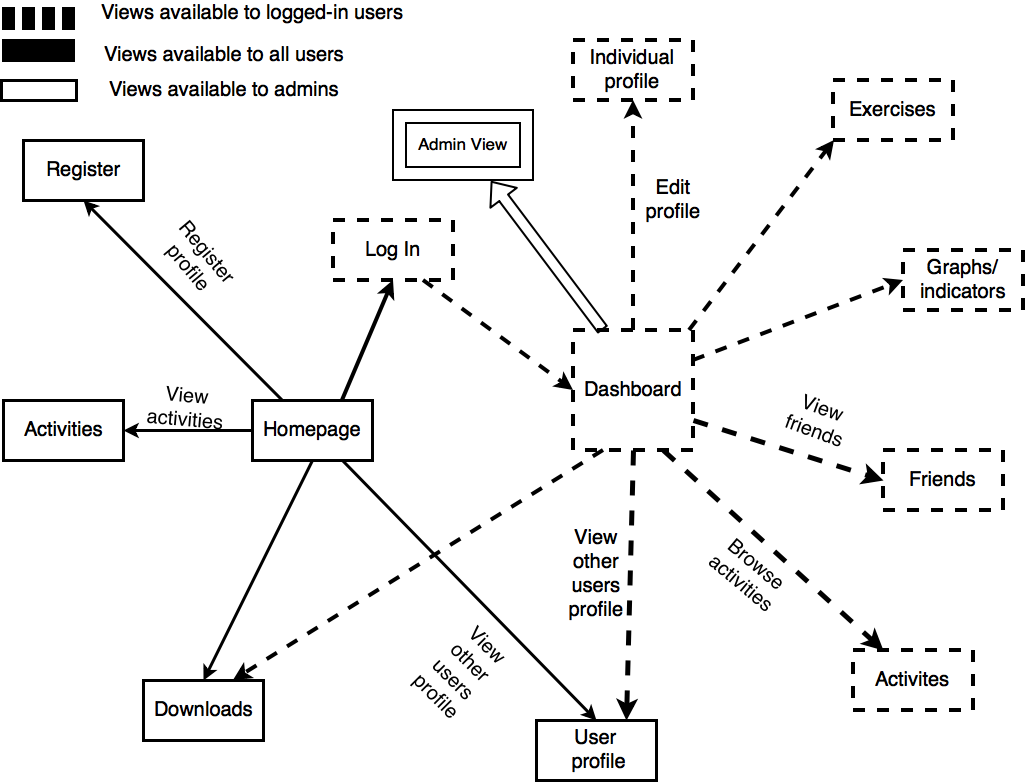
\includegraphics[scale=0.3]{Figures/StateDiagram.png}
\caption{State Diagram of Web Solution}
\label{fig:WebState}
\end{figure}


\subsection{State Diagram of Mobile App}
This is the state diagram for the app. The app has limited functionality, as opposed to the web solution.

\begin{figure}[H]
\centering
\includegraphics[scale=0.3]{Figures/AppStateDiagram.png}
\caption{State Diagram of App Solution}
\label{fig:AppState}
\end{figure}